\section{System Design and Architecture}
In this section, we describe \system{}, which orchestrates updates to feature tables with adaptation to feedback. Downstream clients query the feature tables through the \system{} client so that \system{} can track query access patterns and also post feedback to \system{} once prediction labels are observed. \amit{Downstream clients query the feature tables through and post feedback to the \system{} client so that \system{} can track query access patterns and the quality of its output}
\sarah{more intuition on the idea of staleness vs. regret?}

% \begin{figure}[t]
% \centering
% 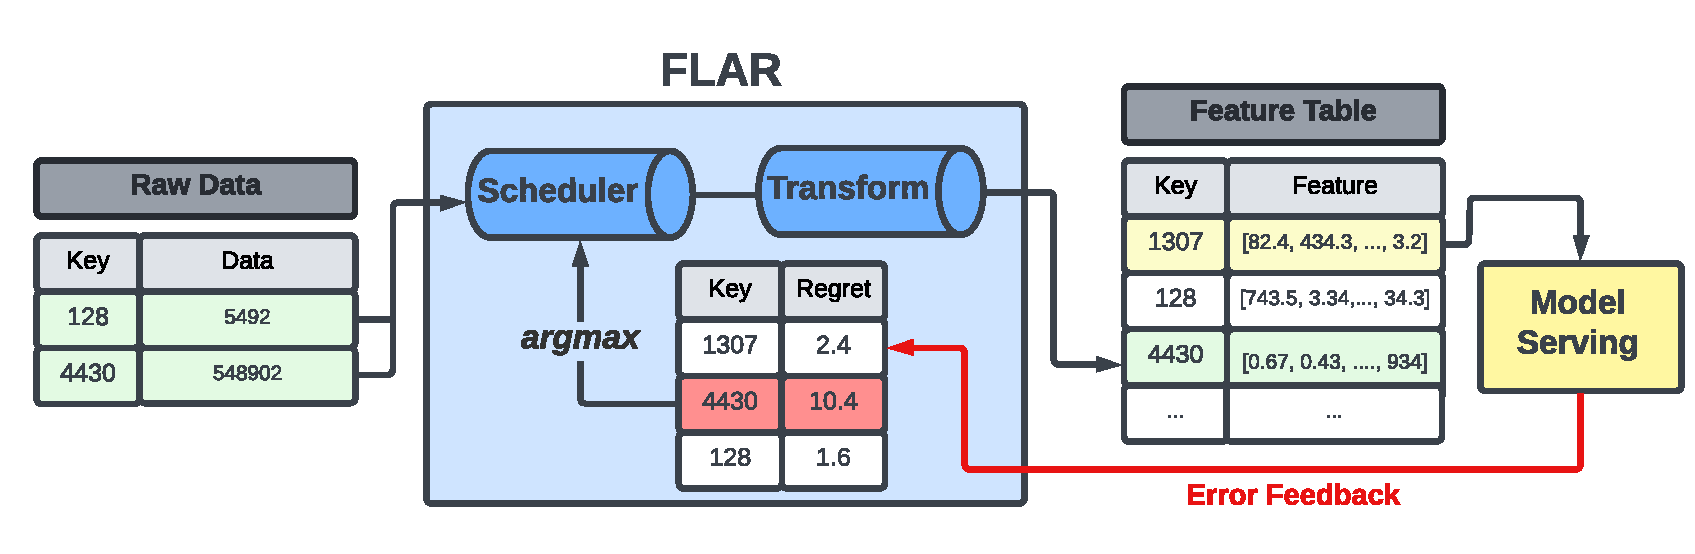
\includegraphics[width=8cm]{ralf/figures/architecture1.pdf}
%  \caption{Overview of a single shard of \system{} Server.}

%  \kevin{Typo in the text above blue box: FLAR -> RALF}
% \label{f:architecture}
% \end{figure}




\label{s:design}
\natacha{It'd be nice to have an overview of what you're going to talk about and even an architecture design "intro". At this point, I'm still unsure what \system{} is}



\natacha{What's the link between shared computation and what we were talking above. Is this a new design? Is is standard feature store architecture??}

\begin{figure}[t]
    \begin{lstlisting}[
language=Python, 
caption=Defining a maintained feature table of user embeddings with RALF. , 
escapechar={|},  
basicstyle=\small,
commentstyle=\color{blue}\sffamily,
stringstyle=\color{red}\sffamily,
numberstyle=\color{gray}\sffamily,
label={lst:api}
]
# Source table 
source = ralf.tables.kafka_source(topic="user_data")

# Queryable feature table 
embedding = source
    .map(UserEmbeddingModel, model_file="model.pt")
    .as_queryable("user_features")
    .set_replicas(4)
    .set_default_error(0.01)
\end{lstlisting}

 
    \begin{lstlisting}[
language=Python, 
caption=Example of a downstream application serving predictions using queried feature values and posting error feedback once the result is observed. , 
escapechar={|},  
basicstyle=\small,
commentstyle=\color{blue}\sffamily,
stringstyle=\color{red}\sffamily,
numberstyle=\color{gray}\sffamily,
label={lst:model_scheduler}
]
class CartAbandonmentModel:
    client = ralf.client(table="user_features")
    cache = {}

    # serve prediction requests 
    def predict(user_id, cart_id): 
        feature, fid = client.get(user_id)
        cache[cart_id] = {
          "pred": model.predict(feature, cart_id),
          "feature_id": fid, 
          "feature_key": user_id
        }
        return cache[cart_id]
        
    # post feedback when label is received 
    def on_label(cart_id, checkout: bool):
        error = MSE(cache[cart_id]["pred"], checkout)
        client.feedback(
          key=cache[cart_id]["feature_key"],
          feature_id=cache[cart_id]["feature_id"],
          error=error
        )
\end{lstlisting}
\end{figure}

% TODO: fix this later
%\RestyleAlgo{ruled}
%\begin{algorithm}[t]
%\caption{Choosing next key to update}\label{alg:choose_key}
%\KwData{List of feedback $F[k]$ for key $k$, $pendingKeys$, $processingKeys$}
%\KwResult{Selected key $k$ to process updates for next.}
%$chosenKey \gets -1$\;
%$maxRegret \gets -1$\;
%\For{$k \in pendingKeys$}{
%$regret = F[k].sum()$\Comment*[r]{Calculate regret}
%
%\If{$regret \ge maxRegret$}{
%$maxRegret\gets regret$\;
%
%$chosenKey\gets k$\Comment*[r]{Update chosen key}
%}
%}
%$F[chosenKey] = []$\Comment*[r]{Clear key feedback}
%$pendingKeys.remove(key)$\;
%$processingKeys.append(key)$\Comment*[r]{Key is processing}
%\Return chosenKey
%\end{algorithm}

%
%\subsection{Operators for Featurization}
%\label{ss:design:operators}
%
\subsection{\system{} Server}
\natacha{What you're describing here doesn't seem to be an an API, but a design?}
\system{} orchestrates data updates to maintain feature values. We show an example of defining a maintained feature table with \system{} in Listing \ref{lst:api}. 
%We show a high-level overview of \system{} in \cref{f:architecture}. 
\system{} schedules and processes data updates to compute new values for the feature table using the specified feature transformation. In addition, \system{} receives queries and error feedback from the client in order to track feature access patterns and quality. \system{} requires a feedback loop: a downstream model that queries feature values must post the observed error for the corresponding key back to the server. This data is used by the scheduler to help decide which key to update next.


\subsubsection{Transformation}
Feature transformations are defined by user definted functions (UDFs) which can maintain state and define an \textit{on\_event} function, which define how to transform a data update from the raw data table to a data update to the feature table. We show an example transformation in Listing \ref{lst:api}. These transformations are implemented as Ray actors, so \system{} relies on Ray for concurrency and fault tolerance.

\subsubsection{Scheduling}
Pending updates are scheduled by \system{} with the scheduler, which chooses the next key to update. The scheduler receives error feedback from downstream models, and uses this to update a table tracking estimated cumulative regret per key. This table is used to select the key with the highest estimated regret. 
The chosen key and corresponding data passed to the transformation.

\subsubsection{Scaling}
\system{} scales to large cardinality datasets by sharding keys across multiple replicas, which each replica can run on separate processing across a single or multiple machines. Each replica has a separate scheduler and error table to avoid coordination.  


%Similar to existing streaming systems, \system{} defines a computation pipeline as a DAG of operators over an incoming stream of data. The output from the computation pipeline represents updates to some materialized feature view, for which we accumulate feature store regret. Each operator in \system{} has scheduling queue for updates, which selects keys with maximal regret. \system{} additionally provides a simple API for downstream applications to query features and post error observations, so that \system{} can allocate feature updates to better optimize for downstream accuracy. 


%\system{}'s API defines featurization pipelines in terms of a DAG of \textit{feature tables}, where each feature table is defined in terms of terms of an operator and one or more input (i.e. parent) feature tables. Feature tables can be make externally queryable through an HTTP interface, and are incrementally updated as new data is streamed into the pipeline. We show an example definition of a feature table in Listing \cref{lst:api}.
%Similar to streaming dataflow systems, \system{} consists of a set of operators chained into a DAG.
%
%
% For example, a featurization pipeline which detects anomalies across a rapidly-changing time series
% (\cref{ss:evaluation:time-series-decomposition}) benefits more
% from a smaller window slide size compared to a stable time series.
% \peter{Consider adding a small experiment to elaborate on/quantify this}
% \sarah{Maybe we could improve figure 2 and reference it here, since it's showing how some time series in the yahoo dataset need very few re-fits}
% %
% The smaller slide size generates more frequent updates, which enables the rapid detection of anomalous changes
% in the time series by downstream operators.
% %
% On the other hand, generating more updates results in more work for downstream operators which may
% run expensive anomaly detection models.
% %
% Because time series for different keys may change at different rates, \system{}'s window operator will
% re-configure each key's window configuration in order to find the ideal trade-off between cost
% and delay in anomaly detection by optimizing the latency-aware feature store accuracy.
% \natacha{This paragraph feels a little strange as it sounds like you didn't have Section 3, and you don't talk about Section 3 at all here. Presumably, isn't the reason why you support per-key window configuration a response to the "findings" you made in Section 3? }
%
% Thus, dynamically adjusting per-key window slide size at runtime can balance compute costs for
% timely anomaly detection by optimizing the latency-aware feature store accuracy.
%

%

%

%\system{} innovates on both the window operator and map operator. 

% \myparagraph{Window Operators}  While traditional windowing operator only allow setting a fixed sized window for the entire stream, \system{}'s windowing operator allow per-key window configuration. For example, in the anomaly detection model use case \kevin{explain earlier what this is}, a time series that's rapidly changing would benefit more from smaller sliding size for a sliding window operator as compare to a very stable time series. For rapidly changing time series, maybe we should emits the sliding window every 2 records to capture any recent changes; while for a stable time series, we can just emits a sliding window every 128 records \kevin{is this very application specific?}. The smaller the slide size, the more records that the downstream operators need to process, therefore increase the compute cost; but smaller the slide size also means we will be capture the freshest data in downstream operators and drive up accuracy. Therefore, *per-key window configuration* allows \system{} to balance compute cost and feature accuracy intelligently. This feature can be implemented as custom windowing operator in traditional streaming dataflow system, however \system{} made it built in and as a first class primitive.
% \sarah{this per-key thing applies to all operator scheduling parameters though, right?}

\subsection{\system{} Client}
The \system{} client is used by downstream applications to query \system{} for features and to post feedback. We show an example of a downstream application in Listing \ref{lst:model_scheduler}, which queries the client for feature values to predict the likelihood of cart abandonment. For applications where true labels are later provided, the application can also post feedback to the client to inform future scheduling the decisions. The feedback takes in the key of queries feature, the queried feature version, and the error of the resulting prediction. Feedback is posted to \system{}, which tracks error feedback for current feature versions on the feature view.  

\subsection{Scheduling Policy}
\label{ss:design:scheduler}
%
\system{} schedules feature updates with Regret-Proportional scheduling, that is, prioritizing updates to keys with the largest \textit{cumulative regret}. The cumulative regret is calculated by tracking the reported error for predictions made using the current feature version stored in the table, and then selecting the key with the largest cumulative regret (as shown in Algorithm \ref{alg:choose_key}). Once a key is chosen, the prior feedback and queue for the key are both cleared, and the key is marked as being processed and locked until the new feature value is computed. The scheduler tracks a list of \textit{pendingKeys}, the list of keys with new data updates, and \textit{processingKeys}, the list of keys where new features are currently being computed. Keys are selected from \textit{pendingKeys}, and once selected, are removed from \textit{pendingKeys} and added to \textit{processingKeys}. Keys in \textit{processingKeys} cannot be chosen again by the scheduler until they are removed once the featurization update is complete - this is to prevent duplicate updates to keys while they are still processing. 


\subsection{Implementation}
\label{ss:design:implementation}
%
\jmh{It's a missed opportunity not to do this in a DBMS with UDFs like Postgres, and talk about materialized views. If you had done so, you'd have a very VLDB-friendly exposition of the APIs, clean example code, clear view materialization opportunities, etc.}
%
%
We construct a full prototype of \system{} in about 1,500 lines of Python code.
%
Our prototype is built atop Ray~\cite{ray}, because many
popular featurization and machine learning libraries (e.g., Tensorflow~\cite{tensorflow})
use Python, and Ray is designed to support machine learning workloads.
%
We emphasize that \system{} is a set of ideas for accuracy-aware featurization, and
can be implemented on several systems. 
% In particular, \system{} can also be implemented as an algorithm to optimize materialized view maintenance in traditional relational database. We chose 

% To show the generality of our contributions, we also provide a reference implementation
% in Timely Dataflow~\cite{timely-dataflow-book}.
%
%
%\myparagraph{Ray prototype}
%

%\jmh{To me the only value of the multiple implementations is to convince the skeptical systems reader that you've solved the problem in a portable way. See my comment below in related work. I wouldn't dwell on evaluating Ray vs Timely vs Noria. Phooey. Now, if one of them lacks the expressivity you need to do the right thing, DO bring that up here, but don't run an evaluation to establish an expressivity problem. By contrast, if one of them is more efficient---e.g., provides a faster update rate---is that really pertinent to your contribution of reframing the feature store freshness problem? Or is it just kind of "System X is more efficient at the class of queries you see here than System Y", but it's not fundamental -- these queries could be tuned up in System Y orthogonal to our techniques. I care more about you characterizing that class -- and then letting the systems optimize for it later if they choose. Finally, there are many systems here you're not evaluating that can express this stuff---notably many database engines---which makes this feel to me like pandering to a narrow audience and its myopia. In the real world I might want to use Snowflake or a high-performance main-memory database; I'm probably not gonna use Noria or Timely. Independent of these pragmatics, why does this paper care anyhow? I feel like you're soiling your beautiful big idea of ``it's the application metric that matters, stupid''  with other people's obsession with system internals of research prototypes. (Grumpy database guy signing off!)}

% \system{} is a set of ideas that bring ML feature quality awareness into streaming dataflow system. It it agnostic to any underlying systems. For this paper, we implemented a prototype system on Ray and a comparison system on Timely Dataflow. We chose to implemented on Ray because it's easy to integrate Python based featurization pipeline and machine learning libraries into the streaming pipeline.
% 
% For the Ray prototype implementation, each operator runs on Ray Actors. Each operator can be sharded by record key. Sharding makes it easy to horizontally scale out the processing throughput. We then use Ray's actor call as RPC mechanism to send records among the operators. 
%
% For the timely dataflow implementation,

% \myparagraph{Offline planner}
% The offline planner was built using an off-the-shelf discreate event simulation library, simpy \cite{matloff2008introduction}. We use the simulation library to generate traces with samples of production workload and compute its accuracy score. To optimize the featurization policies across keys, we use a mixed integer linear program solver (OR-tools \cite{van2014or}) to optimize the final feature policies. The linear program is written to solve for the lowest cost combination of feature policy per key, under a compute budget constraint.
